\section{Fault Trees}

\subsection{Static Fault Trees}

\begin{frame}
\frametitle{Static Fault Trees}
\begin{tikzpicture}[fault tree, global scale=0.7]
\node (r) [event] {Low Power}
    child {
      node (both) [event] {Both inputs fail}
      child { node (a1) [event] {A fails} } 
      child { node (b1) [event] {B fails} }
    }
    child {
      node (si) [event] {One input fails and the switcher fails}
      child { node (s) [event] {Switcher fails}}
      child { 
        node (oneinput) [event] {One input fails}
        child { node (a2) [event] {A fails} }
        child { node (b2) [event] {B fails} }
      }
    };

\node [or gate] (or1) at (r.south) {};
\node [and gate] (and1) at (both.south) {};
\node [and gate] at (si.south) {};
\node [or gate] at (oneinput.south) {};
\node [basic] at (a1.south) {};
\node [basic] at (a2.south) {};
\node [basic] at (b1.south) {};
\node [basic] at (b2.south) {};

\onslide<3>{
\node [above=0.1cm of r] {$(A \land B) \lor (S \land (A \lor B))$};
\node [above=0.3cm of both] {$A \land B$};
\node [above=0.3cm of si] {$S \land (A \lor B)$};
\node [above=0.3cm of oneinput] {$A \lor B$};
}

\onslide<2>{
\node (rdescr) [above right=0.5cm and 0cm of r] {Root event};
\draw (rdescr) edge[->] (r);

\node (interdescr) [above right=0.5cm and 0cm of si] {Intermediary event};
\draw (interdescr) edge[->] (si);

\node (ordescr) [below right=0 and 0.5cm of or1] {OR gate};
\draw (ordescr) edge[->] (or1);

\node (anddescr) [below right=0 and 0.5cm of and1] {AND gate};
\draw (anddescr) edge[->] (and1);

\node (basicdescr) [below right=0.3 and 0.5cm of a1] {Basic event};
\draw (basicdescr) edge[->] (a1);
}

      %child {
      %  node [and gate] {}
      %  child {
      %    node [event] {One input fails and the switcher fails}
      %    child { node [basic] {Switcher fails} }
      %    child {
      %      node [event] {One input fails}
      %      child {
      %        node [or gate] {}
      %        child [basic] {A fails}
      %        child [basic] {B fails}
      %      }
      %    }
      %  }
      %}
\end{tikzpicture}
\end{frame}

\subsection{Dynamic Fault Trees}

\begin{frame}
\frametitle{Dynamic Fault Trees}
\begin{itemize}
  \item Priority AND -- PAND\\
    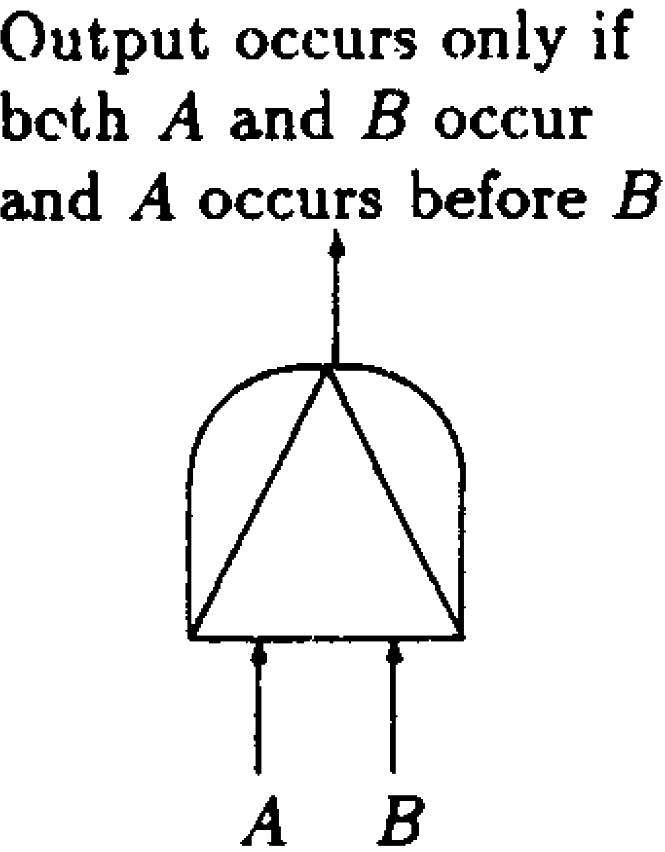
\includegraphics[height=4cm]{pand-dugan}
\end{itemize}
\end{frame}

\begin{frame}
\frametitle{Dynamic Fault Trees}
\begin{itemize}
  \item Cold Spare gate -- CSP\\
    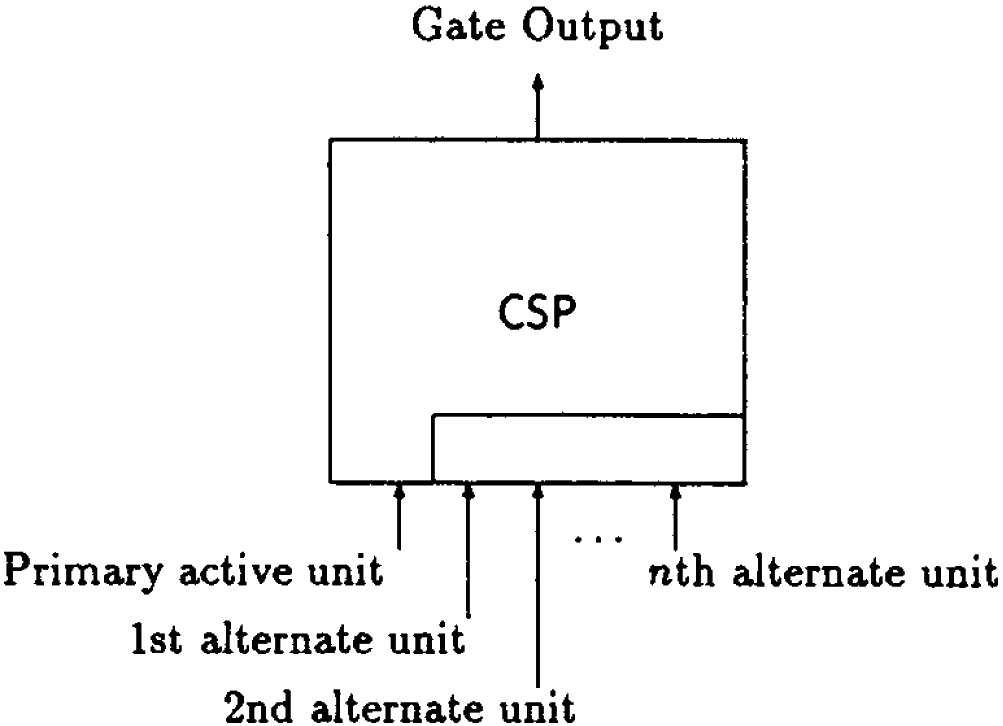
\includegraphics[height=4cm]{csp-dugan}
  \item Example: 4 tires, 1 spare
\end{itemize}
\end{frame}

\begin{frame}
\frametitle{Dynamic Fault Trees}
\begin{itemize}
  \item Sequence Enforcing gate -- SEQ (dummy output)\\
    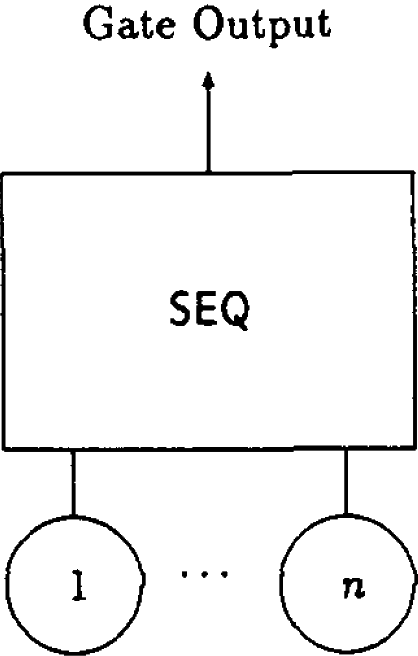
\includegraphics[height=4cm]{seq-dugan} 
  \item Events are forced to occur in a specific order
\end{itemize}
\end{frame}

\begin{frame}
\frametitle{Dynamic Fault Trees}
\begin{itemize}
  \item Functional Dependency gate -- FDEP (dummy output)\\
    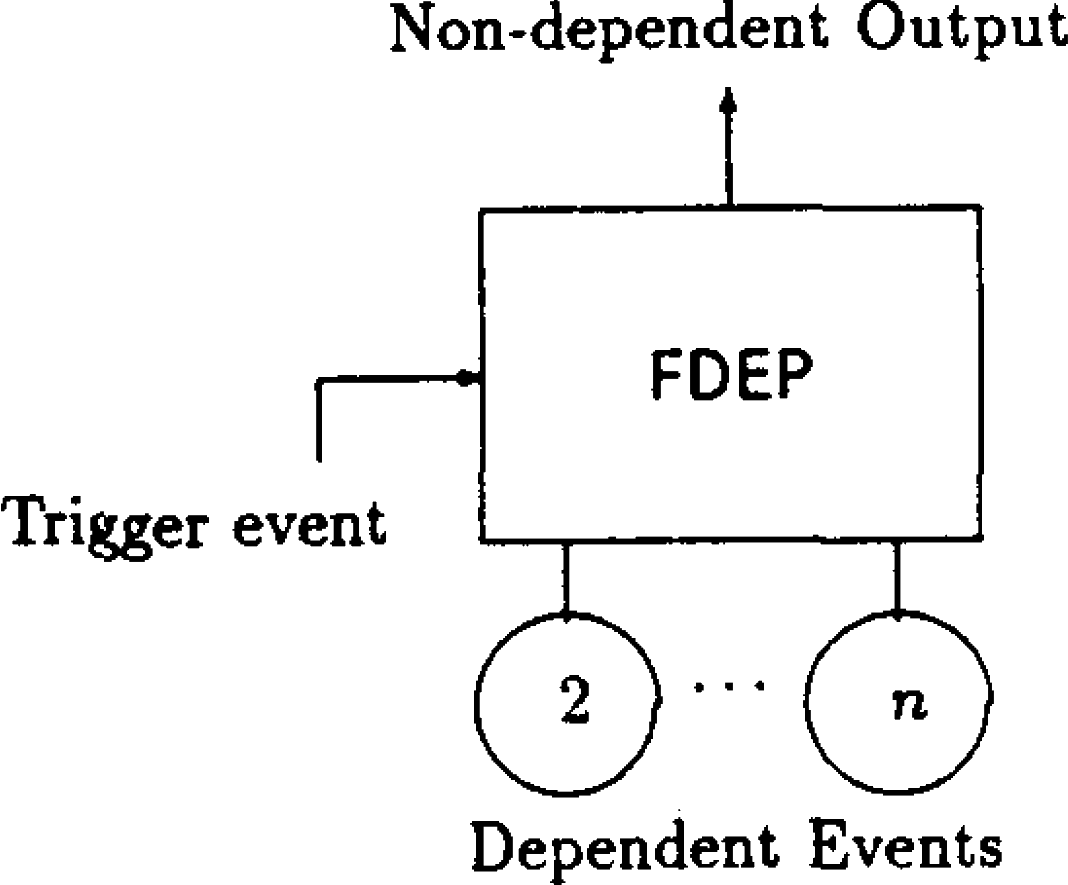
\includegraphics[height=4cm]{fdep-dugan}
  \item Dependent events are forced to occur when the trigger events activates;
  \item Otherwise they are independent.
\end{itemize}
\end{frame}

\begin{frame}
\frametitle{Relevant DFT gates}
\begin{itemize}
  \item SEQ is expressible in terms of CSP.
  \item For DFT, the relevant gates are then PAND, FDEP and CSP. 
\end{itemize}
\end{frame}

\subsection{Temporal Fault Trees}

\begin{frame}
\frametitle{Temporal Fault Trees}
\begin{itemize}
  \item Priority AND gate -- PAND\\
  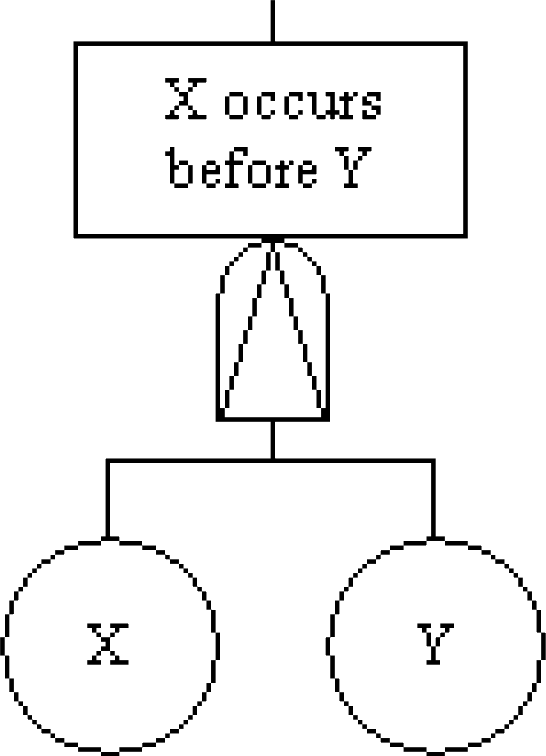
\includegraphics[height=4cm]{pand-walker}
\end{itemize}
\end{frame}

\begin{frame}
\frametitle{Temporal Fault Trees}
\begin{itemize}
  \item Priority OR gate -- POR\\
  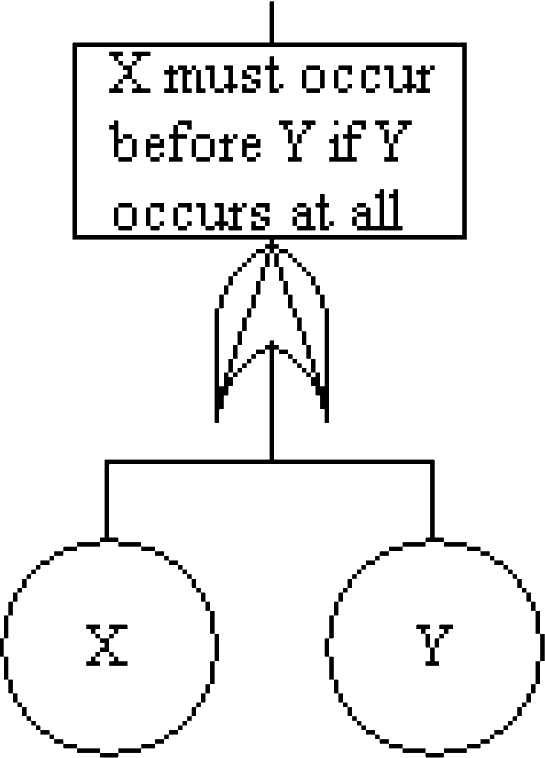
\includegraphics[height=4cm]{por-walker}
\end{itemize}
\end{frame}

\begin{frame}
\frametitle{Temporal Fault Trees}
\begin{itemize}
  \item Simultaneous gate -- SAND\\
  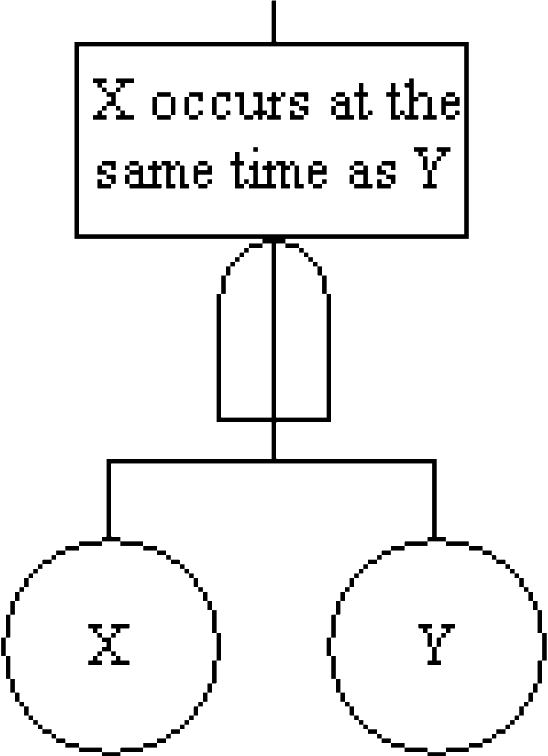
\includegraphics[height=4cm]{sand-walker}
\end{itemize}
\end{frame}

\subsection{TFT formalization}

\begin{frame}
\frametitle{TFT algebra}

\begin{itemize}
  \item Every event has a sequence number.
  \item There aren't gaps between events' sequence numbers. Ex.: for events $A$ and $B$, if $A$ has sequence number $1$, then $B$ has sequence number $0$, $1$ or $2$. It cannot have sequence number $3$ or higher.
  \item Sequence number $0$ means that the event hasn't occurred.
  \item Temporal Truth Tables helps understand TFT operators:
  {
  \scriptsize
  \begin{tabular}{c|c|c|c|c|c|c}
  A & B & AND & OR & PAND & POR & SAND\\
  \hline
  0 & 0 & 0 & 0 & 0 & 0 & 0\\
  \hline
  0 & 1 & 0 & 1 & 0 & 0 & 0\\
  \hline
  1 & 0 & 0 & 1 & 0 & 1 & 0\\
  \hline
  1 & 1 & 1 & 1 & 0 & 0 & 1\\
  \hline
  1 & 2 & 2 & 1 & 1 & 1 & 0\\
  \hline
  2 & 1 & 2 & 1 & 0 & 0 & 0\\
  \hline
  \end{tabular}
  }
  \item Simultaneity is allowed.
\end{itemize}

\end{frame}

\begin{frame}
\frametitle{TFT operators}

\begin{itemize}
  \item PAND: 
    \begin{itemize}
      \item Symbol: $<$
      \item Sequence value: $S(A<B) = S(B)$
      \item Logic: $A$ and $B$ occur and $A$ occurs before $B$
    \end{itemize}
  \item SAND: 
    \begin{itemize}
      \item Symbol: $\&$
      \item Sequence value: $S(A\&B) = S(A) = S(B)$
      \item Logic: $A$ and $B$ occur at the same time
    \end{itemize}
  \item POR: 
    \begin{itemize}
      \item Symbol: $|$
      \item Sequence value: $S(A|B) = S(A)$
      \item Logic: either $A$ occurs and $B$ does not, or both occur and $A$ occurs first
    \end{itemize}
\end{itemize}
\end{frame}

\begin{frame}
\frametitle{TFT algebra issues}

\begin{itemize}
  \item A reduction algorithm uses dependency trees that makes the analysis infeasible for trees with eight or more basic events.
  \item Due to the use of sequence numbers, PAND is not associative: $X<Y<Z \ne X<(Y<Z) \ne (X<Y)<Z$ 
  \item It redefines all traditional Boolean operators and laws using sequence numbers 
  \item The algebra does not allow NOT gates
    \begin{itemize}
      \item<2-> There are cases where NOT gates may cause non-coherent analysis, and cases where it is necessary.
    \end{itemize}
\end{itemize}
\end{frame}

\subsection{DFT formalization}

\begin{frame}
\frametitle{DFT algebra}

\begin{itemize}
  \item Uses a continuous \emph{date-of-occurrence} function ($d(t)$) which is $0$ while its event hasn't occurred, or is $1$ if it has occurred
  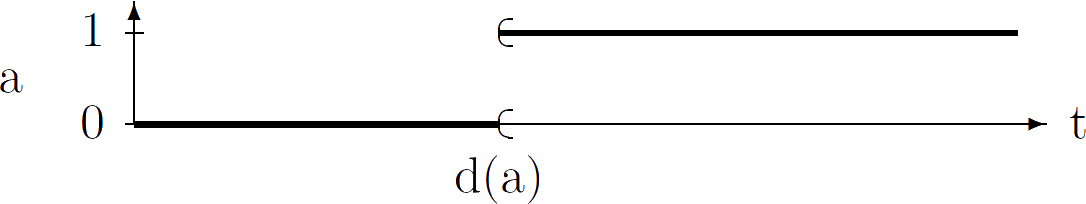
\includegraphics[height=1cm]{date-of-occurrence-merle}
  \item All relevant DFT gates can be rewritten in terms of three operators: 
    \begin{itemize}
      \item non-inclusive before ($\nibefore$): similar to TFT algebra's POR gate.
      \item simultaneous ($\simultaneous$): similar to TFT algebra's SAND gate.
      \item inclusive before ($\ibefore$): a ``shortcut'' (all laws are proved) to \emph{non-inclusive before or simultaneous}.
    \end{itemize}  
  \item Simultaneity is allowed, but probabilistically impossible.
\end{itemize}
\end{frame}


\begin{frame}
\frametitle{DFT algebra operators}

\begin{itemize}
  \item Non-inclusive before:
  $
  \doo (a \nibefore b) =
  \begin{cases}
  \doo(a) & \doo(a) < \doo(b)\\
  +\infty & \doo(a) = \doo(b)\\
  +\infty & \doo(a) > \doo(b)\\
  \end{cases}
  $
  \item Simultaneous:
  $
  \doo (a \simultaneous b) =
  \begin{cases}
  +\infty & \doo(a) < \doo(b)\\
  \doo(a) & \doo(a) = \doo(b)\\
  +\infty & \doo(a) > \doo(b)\\
  \end{cases}
  $
  \item Inclusive before:
  $
  \doo (a \ibefore b) =
  \begin{cases}
  \doo(a) & \doo(a) < \doo(b)\\
  \doo(a) & \doo(a) = \doo(b)\\
  +\infty & \doo(a) > \doo(b)\\
  \end{cases}
  $
\end{itemize}
\end{frame}

\begin{frame}
\frametitle{DFT algebra issues}

\begin{itemize}
  \item It redefines all traditional Boolean operators and laws using the date-of-occurrence function
  \item The algebra does not allow NOT gates
  \item It is not clear how to reduce the structure function to obtain its minimal canonical form (all analysis are based on this form)
\end{itemize}
\end{frame}